\section{Packages description}
\label{sec:Packages}


\subsection{Packages structure}
Despite the fact that we recommend users to install the complete COMPSs Framework, we have built different packages to allow users
customize as maximum as possible their installation. Figure \ref{fig:compss_packages_debian} illustrates the COMPSs 
packaging structure and its internal dependencies. 
\begin{figure}[ht!]
  \centering
    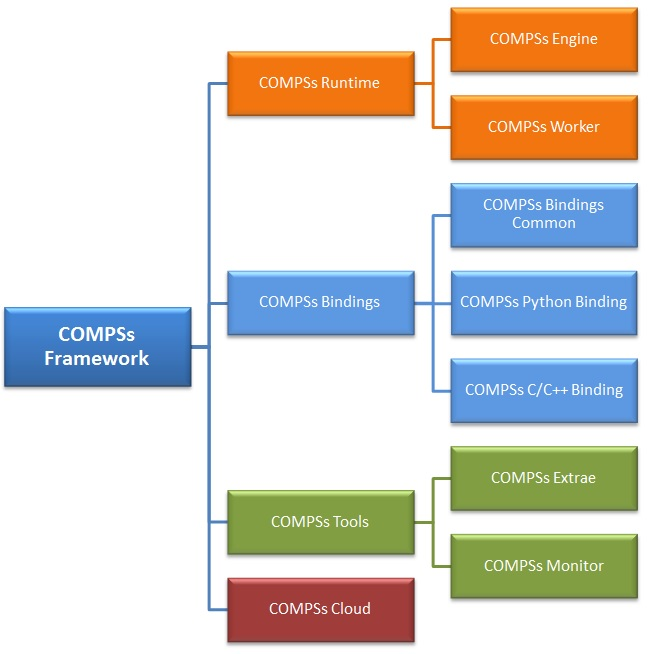
\includegraphics[width=0.75\textwidth]{./Sections/02_Packages_Description/Figures/compss_packages.jpeg}
    \caption{COMPSs packaging structure}
    \label{fig:compss_packages_debian}
\end{figure}

\newpage

\subsection{Packages Dependencies}
\label{subsec:packages_dependencies}
Next we provide a list of dependencies for each COMPSs package. The exact names may vary depending on 
the Linux distribution but this list provides a general overview of the COMPSs dependencies. For specific information about
your distribution please check the \textit{Depends} section at your package manager (apt, yum, zypper, etc.).

\bgroup
  \def\arraystretch{1.5}
  \begin{center}
    \begin{tabular}{ p{6cm} | p{10cm} }
    COMPSs Framework 		& compss-runtime, compss-bindings, compss-tools, compss-cloud \\ \hline 
    COMPSs Runtime 		& compss-engine, compss-worker \\ \hline  
    COMPSs Engine 		& openjdk-8-jre, graphviz, xdg-utils \\ \hline 
    COMPSs Worker 		& openjdk-8-jre \\ \hline 
    COMPSs Bindings 		& compss-bindings-common, compss-c-binding, compss-python-binding \\ \hline 
    COMPSs Bindings Common 	& compss-engine, libtool, automake, build-essential \\ \hline 
    COMPSs Python Binding 	& compss-bindings-common, python ($>= 2.7$), libpython2.7 \\ \hline 
    COMPSs C/C++ Binding 	& compss-binding-common, libboost-serialization-dev, libboost-iostreams-dev, libxml2-dev, csh \\ \hline 
    COMPSs Tools 		& compss-extrae, compss-monitor \\ \hline 
    COMPSs Extrae 		& compss-engine, libxml2 ($>= 2.5$), libxml2-dev ($>= 2.5$), gfortran, papi \\ \hline 
    COMPSs Monitor 		& compss-engine \\ \hline 
    COMPSs Cloud 		& compss-engine    
    \end{tabular}
  \end{center}
\egroup

\subsection{Optional Dependencies}
For the Python binding it is also recommended to have \verb|dill| and \verb|guppy| installed. The \verb|dill| package increases
the variety of serializable objects by Python (for example: lambda functions), and the \verb|guppy| package is needed to use the \verb|@local|
decorator. Both packages can be found in pyPI and can be installed via \verb|pip|.
